\documentclass{beamer}

% Use metropolis theme
\usetheme[progressbar=frametitle]{metropolis}
\usepackage{minted}
\usepackage{subfig}
\usepackage{hyperref}

\title{How to Use Python and Mathematical Modeling to Better Understand the Impact of Electricity Pricing on Consumption}

% \date{November 2, 2023}
\date{\today}
\author{Saba Nejad}
% \institute{PyData NYC 2023}

\begin{document}
\maketitle

\section{Outline}

\begin{frame}{Overview of the Talk}
  \begin{itemize}
  \item Introduce the Problem Space; Define Terminology
  \item Introduce the Trial and the Dataset
  \item Mathematical Model
  \item Data Prep, Cleaning, Processing
  \item Results
  \end{itemize}
\end{frame}

\section{The Background}

\begin{frame}{The Power Grid}
  \begin{itemize}
    \item<+-> Electricity is unique in that its \textbf{storage is prohibitively costly}. As a result, \textbf{supply must at least meet demand} at all times. 
    \item<+-> (Regional / Independent) \textbf{System Operators}: Resposible for reliable delivery of electricity to consumers.
    \begin{center}
      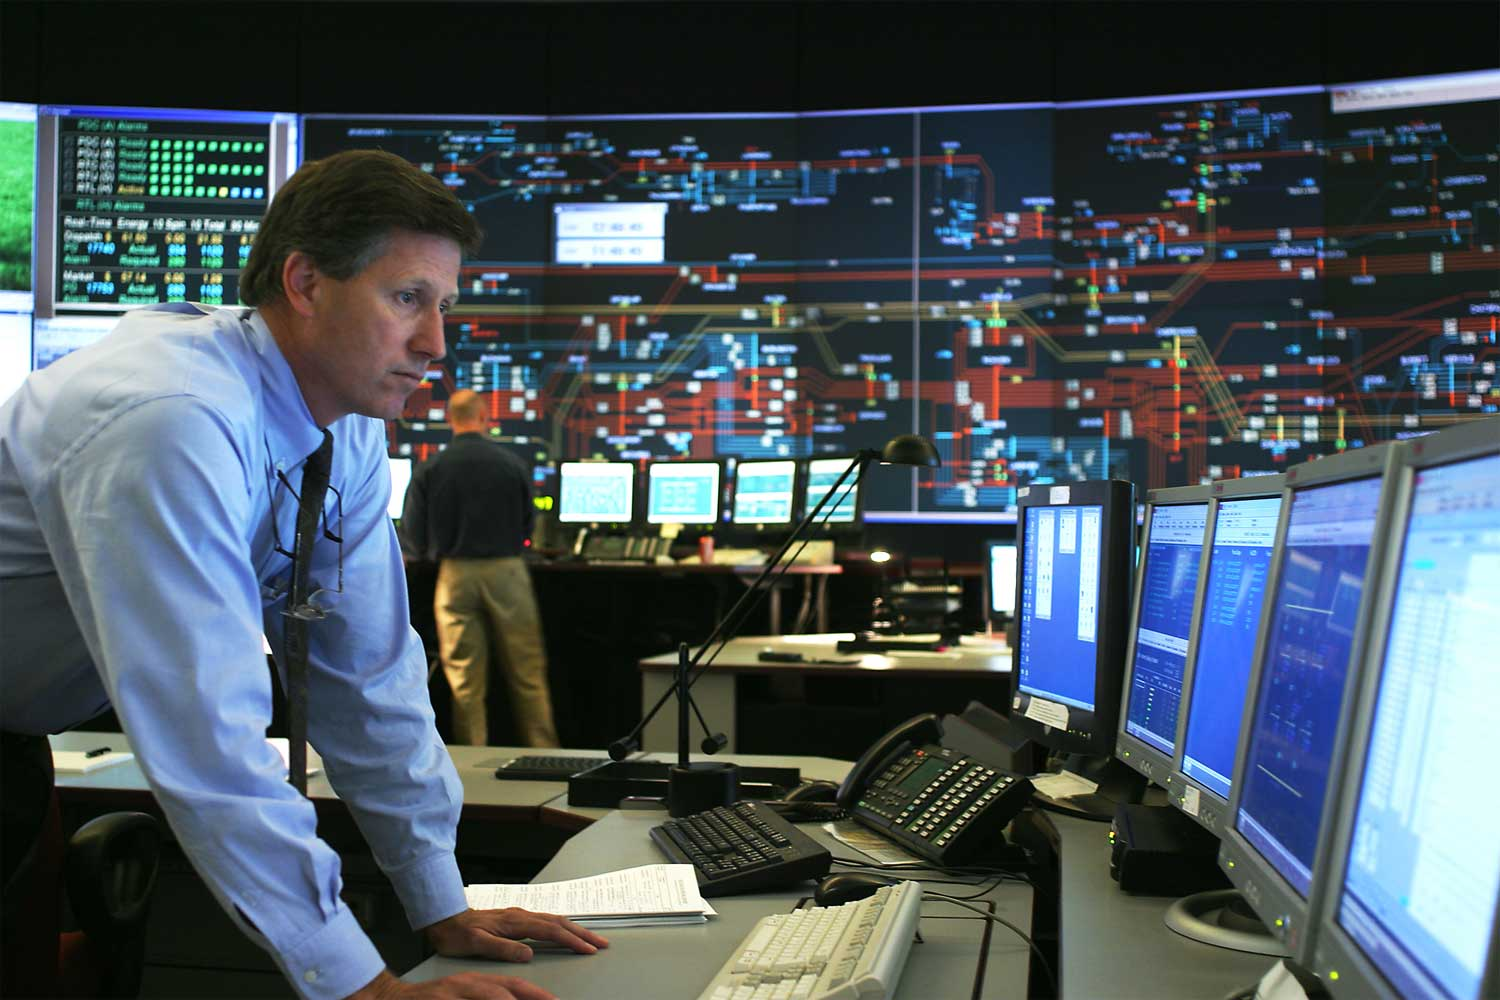
\includegraphics[width=0.65\textwidth]{images/iso-control-room.png}
    \end{center}
  \end{itemize}
\end{frame}

\begin{frame}{Demand Response}
  \begin{itemize}
    \item (Dynamic) Time of Use Pricing (dToU)
    \begin{itemize}
      \item Assumption 1: Demand can be shifted around.
      \item Assumption 2: Players are price sensitive ie there's correlation between demand and price.
    \end{itemize}
  \end{itemize}
  \vspace{0.5cm}
  \centering
  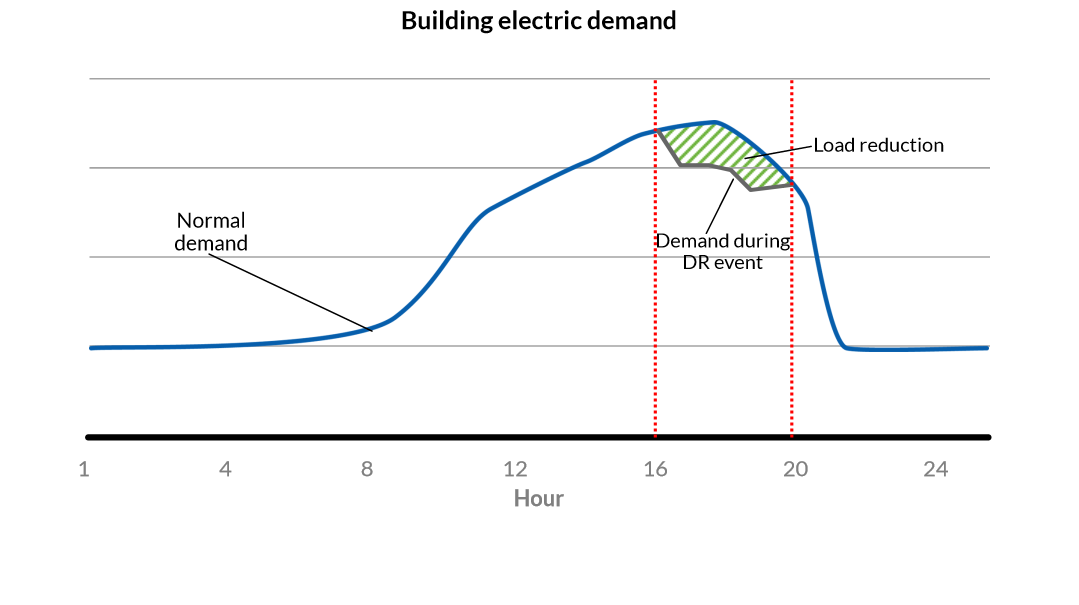
\includegraphics[width=0.85\textwidth]{images/demand-response.png}
\end{frame}

\section{The Data}

\begin{frame}{Low Carbon London Smart Meter Trial}
  \begin{itemize}
    \item<+-> Motivation: The Climate Change Act of 2008 sets the target of reducing carbon emissions to 20\% of 1990 levels by 2050.
    \item<+-> The tariff prices were given a day ahead via the Smart Meter In Home Display or text message.
    \item<+-> Data spans November 2011 and February 2014 (around 167M records); Treatment took place for the calendar year 2013 only.
    \item<+-> Readings were taken at half hourly intervals; discrete socio-economic feature per household included in the data.
    \item<+-> dTou price bands vs static pricing model:
    \begin{table}[]
      \begin{tabular}{|l|l|}
        \hline
        dToU Pricing Model & Static Pricing Model \\ \hline
        High (67.20 p/kWh) & 14.228 pence/kWh \\ \hline
        Normal (11.76 p/kWh) & 14.228 p/kWh \\ \hline
        Low (3.99 p/kWh) & 14.228 p/kWh \\ \hline
      \end{tabular}
    \end{table}
  \end{itemize}
\end{frame}

\begin{frame}{Low Carbon London Smart Meter Trial: Biases?}
  \textbf{The trial is double opt-in}: Households opt into sharing their data with the trial at all, And they opt into the dToU pricing model + certain incentives:
  \begin{itemize}
    \item A guarantee that they will be reimbursed at the end of trial if they are worse off on the dToU tariff than they would have been on their previous tariff.
    \item Assurances regarding how many hours would be charged at the high price band.
    \item \textsterling100 for signing up to the dToU tariff.
    \item Another \textsterling50 for staying on the dToU tariff until the end of trial.
    \item Entry into a prize draw after completion of the post trial survey.
  \end{itemize}
\end{frame}

\begin{frame}{Low Carbon London Smart Meter Trial: Distribution?}
  \begin{figure}
    \centering
    \subfloat[\centering Trial household sample locations overlaid on the borough boundary map of Greater London. Map data from the Greater London Authority. This shows that the treatment and control group were representative samples of Greater London.]{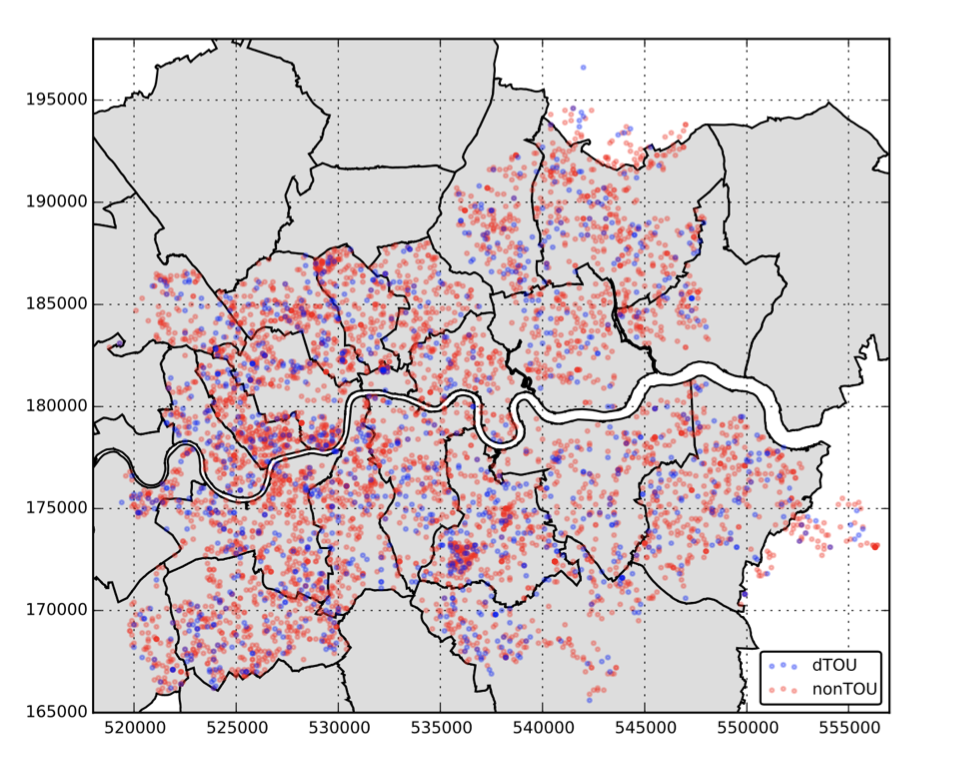
\includegraphics[width=5cm]{images/london-geo-breakdown.png}}
    \qquad
    \subfloat[\centering The treatment and control groups were also representative socio-economic samples of Greater London.]{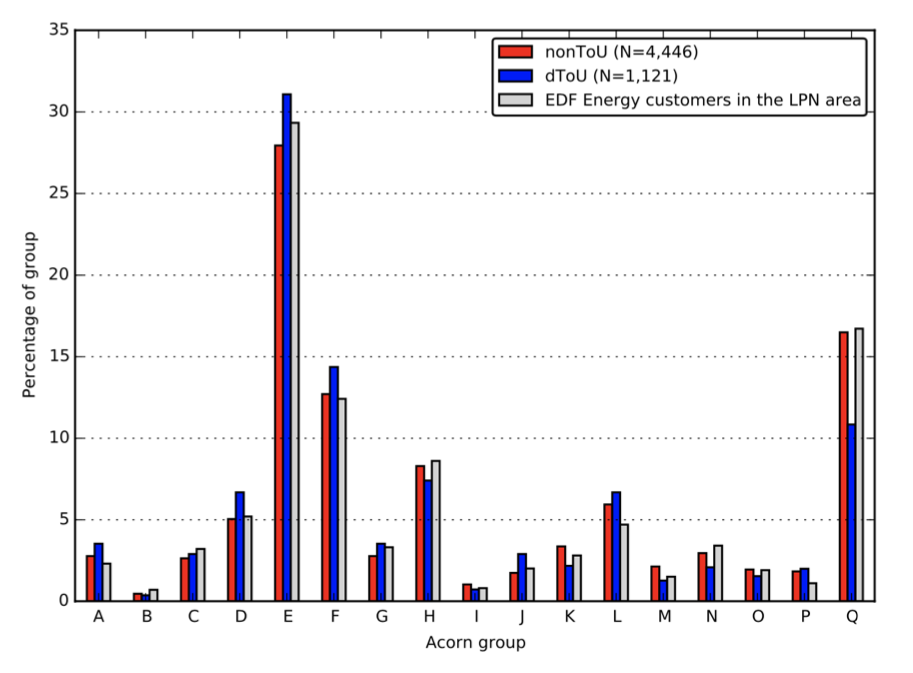
\includegraphics[width=5cm]{images/london-socio-breakdown.png}}
  \end{figure}
\end{frame}

\begin{frame}{Low Carbon London Smart Meter Trial: Missing Data}
  \begin{itemize}
    \item 2012: Users were still onboarding.
    \item 2013: Some users dropped out of both the treatment and the control groups
    \item 5,567 total households participated: 4,500 were in the control group, 1,100 were in the treatment group.
  \end{itemize}
  \vspace{-0.5cm}
  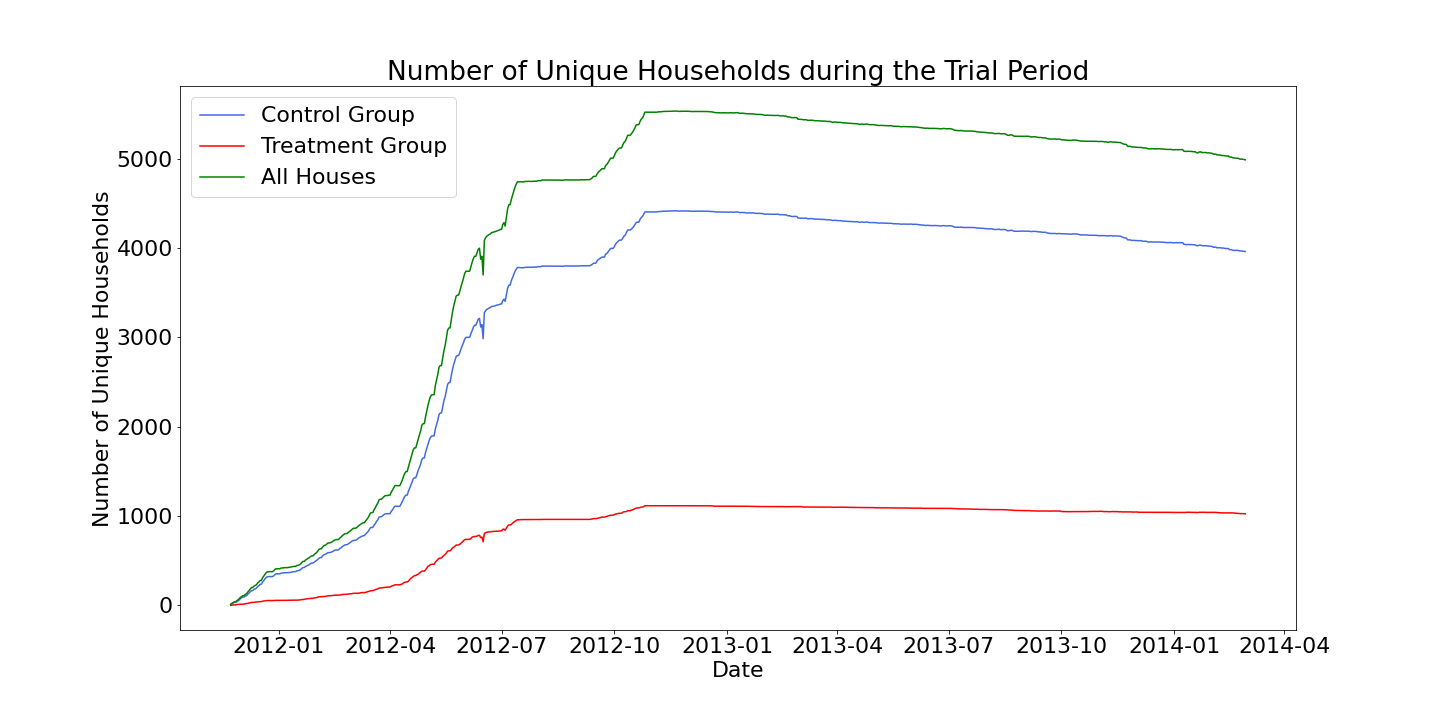
\includegraphics[width=1\textwidth]{images/house-count.png}
\end{frame}

\section{The Math}

\begin{frame}{The Fundamental Problem of Causal Inference (FPCI)}
  \begin{itemize}
    \item<+-> Assume $X \in\{0,1\}$ is a binary causal variable and $Y$ is a response variable (which may be continuous).
    \item<+-> Assume $X$ has a causal effect on $Y$, this implies that the value of $Y$ we observe depends on the value of $X$.
    \item<+-> We can define $Y_0$ and $Y_1$ as the values that $Y$ would take if $X$ were equal to 0 and 1 respectively.
    \item<+-> $Y_0$ and $Y_1$ are counterfactuals of one another. Both can never be observed at the same time.
    \begin{itemize}
      \item $Y_i$ := the outcome of interest for unit $i$
      \item $Y_0$ := the value of $Y_i$ for $X=0$ (untreated unit)
      \item $Y_1$ := the value of $Y_i$ for $X=1$ (treated unit)
    \end{itemize}
  \end{itemize}
\end{frame}

\begin{frame}{The Fundamental Problem of Causal Inference (FPCI)}
  \begin{itemize}
    \item<+-> Assume that units are all alike, so $Y_{0 i} \equiv Y_0$ and $Y_{1 i} \equiv Y_1$.
    \item<+-> The causal effect of $X_i$ on $Y_i$ is $T=Y_1-Y_0$, where $T$ stands for Treatment Effect.
    \item<+-> \textit{But what's the issue here?}
    \item<+-> We never observe $Y_1-Y_0$ for a single unit $i$. Instead, we observe
    $$
    Y_i=Y_{1 i} X_i+Y_{0 i}\left(1-X_i\right)
    $$
    That is, we observe $Y_1$ or $Y_0$ but not both.
  \end{itemize}
\end{frame}

\begin{frame}{Solutions Around FPCI}
  \begin{enumerate}
    \item<+-> Temporal Stability \& Causal Transience
    \item<+-> Unit Homogeneity
    \item<+-> Analyze Populations Instead of Units
  \end{enumerate}
\end{frame}

\begin{frame}{Solutions Around FPCI for this Trial}
  \begin{enumerate}
    \item Temporal Stability \& Causal Transience {\color{red}{X}}
    \item Unit Homogeneity {\color{red}{X}}
    \item Estimate causal effects for populations rather than units {\color{green}{\checkmark}}
  \end{enumerate}
\end{frame}

\begin{frame}{Estimate Causal Effects for Populations Rather than Units}
  \begin{itemize}
    \item<+-> Causal Effect for Unit $i$: $T_i=Y_{1 i}-Y_{0 i}$
    \begin{itemize}
      \item \textit{We can't estimate this. Why?}
    \end{itemize}
    \item<+-> Average Treatment Effect for the Treated (ATT): $T^*=E\left[Y_1-Y_0 \mid X=1\right]$
    \item<+-> Average Treatment Effect (ATE): $T^{\dagger}=E\left[Y_1-Y_0\right]$
    \item<+-> \textit{ATE is treatment effect assuming entire population is treated.}
      \begin{itemize}
        \item \textit{What's an example?}
        \item \textit{Which of the two is more important? But how do we estimate it?}
      \end{itemize}
  \end{itemize}
\end{frame}


\begin{frame}{Estimate Causal Effects for Populations Rather than Units}
  To make things more complicated, let's make another estimator.
  \begin{enumerate}
    \item<+-> $\tilde{T}=E[Y \mid X=1]-$ $E[Y \mid X=0]$
  \end{enumerate}
  Is $\tilde{T}$ a good estimator of $T^*$? What is it estimating?
  What change can we make to our population to make this a good estimator?
\end{frame}

\begin{frame}{Estimate Causal Effects for Populations Rather than Units}
  \begin{itemize}
    \item<+-> Assume your treatment and control group had the same expected baseline behavior, and the same counterfactual expected behavior.
    $$
    \begin{aligned}
    & E\left[Y_1 \mid X=1\right]=E\left[Y_1 \mid X=0\right] \\
    & E\left[Y_0 \mid X=1\right]=E\left[Y_0 \mid X=0\right]
    \end{aligned}
    $$
    \item<+-> Let's revisit $$ \begin{aligned}
      T^* & = E\left[Y_1 \mid X=1\right]-E\left[Y_0 \mid X=1\right] \\
          & = E\left[Y_1 \mid X=1\right]-E\left[Y_0 \mid X=0\right] 
    \end{aligned} $$
  \end{itemize}
\end{frame}

\begin{frame}{Estimate Causal Effects for Populations Rather than Units}
  \begin{itemize}
    \item<+-> but what if they aren't exactly the same, this would often hold in the case of an actual treatment. In other words there's a reason for the treatment:
    \item<+-> $$
    \begin{aligned}
    & E\left[Y_1 \mid X=1\right]>E\left[Y_1 \mid X=0\right] \\
    & E\left[Y_0 \mid X=1\right]>E\left[Y_0 \mid X=0\right] .
    \end{aligned}
    $$
    \item<+-> ... let's bring back $\tilde{T}$. 
  \end{itemize}
\end{frame}

\begin{frame}{Estimate Causal Effects for Populations Rather than Units}
  So, if we calculated the contrast $\tilde{T}=E[Y \mid X=1]-E[Y \mid X=0]$ for this unbalanced group, what would we get?
  $$
  \begin{aligned}
  E\left[Y_1 \mid X=1\right]-E\left[Y_0 \mid X=0\right] & =\underbrace{E\left[Y_1 \mid X=1\right]-E\left[Y_0 \mid X=1\right]}_{T^*} \\
  & +\underbrace{\left\{E\left[Y_0 \mid X=1\right]-E\left[Y_0 \mid X=0\right]\right\}}_{\text {Bias }} .
  \end{aligned}
  $$
  (Go to whiteboard and do the rest)
\end{frame}

% Notice that our substitution above of $E\left[Y_0 \mid X=1\right]$ for $E\left[Y_0 \mid X=0\right]$ is justified by the assumption of treatment-control balance in equation (1). If the subjects who didn't receive the treatment are just like those who did but for not having received the treatment, then the contrast between the treated and untreated groups provides an unbiased estimate of the causal effect of the treatment on the treated group (ATT).
% - Returning to our invalid estimator $\tilde{T}$, let's ask how likely is it that the counterfactual outcomes would be balanced among a set of people selected from the population according to whether or not they are currently receiving the treatment. It does not take a great leap of logic to hypothesize that the patients receiving the cholesterol drug are more likely to be suffering from high cholesterol than those who are not taking the drug. This would imply that:


% In words, patients receiving the drug are more likely to suffer from high cholesterol whether or not they are receiving the drug (presumably, they are receiving the drug specifically because they were diagnosed with high cholesterol).


% The first term on the right-hand side of this equation is the true, causal effect of the cholesterol treatment on those who take it (the ATT). The second term is the potential bias that

\section{The Analysis}

\begin{frame}
  Assume matrix $\alpha^{t \times n_c}$ contains control group data, and $\beta^{t \times n_t}$ contains treatment group data. Where $t = 365 \times 48 = 17520$, $n_c$ is the number of households in the control group and $n_t$ is the number of households in the treatment group.
  \begin{align}
    \begin{split}
      \overline{\beta^m_{2012}} &= a \times \overline{\alpha^m_{2012}} + b \\
      \overline{\hat{\beta}^m_{2013}} &= a \times \overline{\alpha^m_{2013}} + b \\
      \overline{\Delta\mbox{treatment}} &= \overline{\beta^m_{2013}} - \overline{\hat{\beta}^m_{2013}}
    \end{split}
  \end{align}
\end{frame}

\begin{frame}{Data Prep, Cleaning, Processing}
  
\includegraphics[width=0.95\textwidth]{images/lcl-raw-files.png}
\end{frame}

\begin{frame}{Data Prep, Cleaning, Processing}
  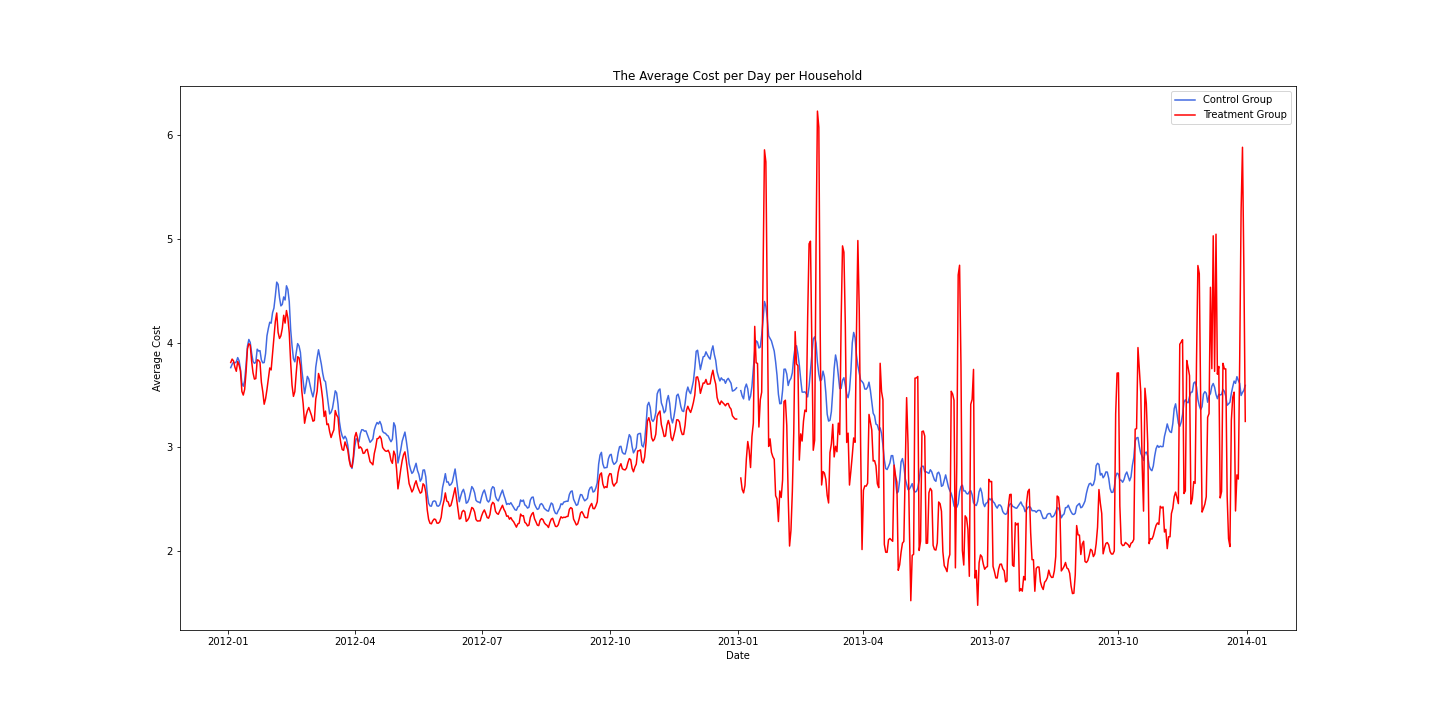
\includegraphics[width=0.95\textwidth]{images/avg-cost-per-day.png}
\end{frame}

\begin{frame}{Data Prep, Cleaning, Processing}
  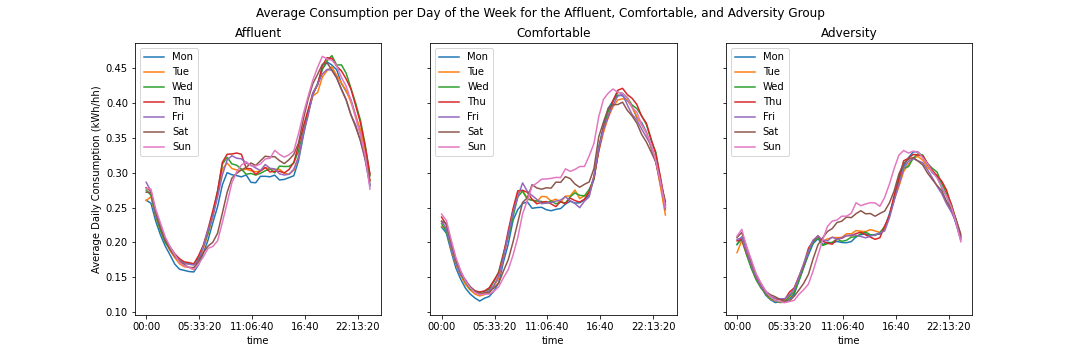
\includegraphics[width=0.95\textwidth]{images/dow-socio.png}
\end{frame}

\section{The Conclusion}

\begin{frame}{What Did We Learn?}
  \begin{itemize}
    \item<+-> A little bit about electricity markets
    \item<+-> Causal Analysis
    \item<+-> How to break down your data to match the mathematical model at hand
    \item<+-> Questions to ask before analysis:
    \begin{itemize}
      \item<+-> How was the data collected? 
      \item<+-> What biases are present?
      \item<+-> How does that impact your analysis and results?
    \end{itemize}
  \end{itemize}
\end{frame}

\begin{frame}{Thank You}
  \begin{itemize}
  \item \url{https://github.com/sabanejad}
  \item \url{https://www.linkedin.com/in/sabanejad/}
  \end{itemize}
\end{frame}

\section{Appendix}

\begin{frame}{Potential Outcomes Framework (Rubin-Neyman Causal Model)}
  Each household $x_i$ has two potential outcomes:
  \begin{itemize}
    \item $Y_0\left(x_i\right)$ is the potential outcome had the unit not been treated (static pricing model): ``control outcome"
    \item $Y_1\left(x_i\right)$ is the potential outcome had the unit been treated (dToU pricing model): ``treated outcome"
  \end{itemize}
  - Conditional average treatment effect for unit $i$ :
  $$
  \operatorname{CATE}\left(x_i\right)=\mathbb{E}_{Y_1 \sim p\left(Y_1 \mid x_i\right)}\left[Y_1 \mid x_i\right]-\mathbb{E}_{Y_0 \sim p\left(Y_0 \mid x_i\right)}\left[Y_0 \mid x_i\right]
  $$
  - Average Treatment Effect:
  $$
  A T E:=\mathbb{E}\left[Y_1-Y_0\right]=\mathbb{E}_{x \sim p(x)}[\operatorname{CATE}(x)]
  $$
\end{frame}

\begin{frame}{Mathematical Model}
\begin{itemize}
  \item Fundamental Problem of Causal Inference: Both outcomes can't be observed for the same household $x_i$.
  \begin{itemize}
    \item Observed factual outcome:
    $$
    y_i=t_i Y_1\left(x_i\right)+\left(1-t_i\right) Y_0\left(x_i\right)
    $$
    \item Unobserved counterfactual outcome:
    $$
    y_i^{C F}=\left(1-t_i\right) Y_1\left(x_i\right)+t_i Y_0\left(x_i\right)
    $$
  \end{itemize}
  \item Solution? Approximate the counterfactual eg close enough to random sample: minimum wage problem, NJ and east PA, Card \& Krueger, 1994.
\end{itemize}
\end{frame}

\begin{frame}
  David Card minimum wage paper: \url{https://davidcard.berkeley.edu/papers/njmin-aer.pdf}
  LCL Experiment \url{https://data.london.gov.uk/dataset/smartmeter-energy-use-data-in-london-households}
\end{frame}

\end{document}